\documentclass[12pt,letterpaper]{article}
\usepackage[bottom=1in, top=1in]{geometry}
\usepackage[]{geometry}

\usepackage[intlimits]{amsmath}
\usepackage[utf8]{inputenc}
\DeclareUnicodeCharacter{2212}{-}
\usepackage{amsfonts,amssymb}
\DeclareSymbolFontAlphabet{\mathbb}{AMSb}
\usepackage{textcomp}

\usepackage{float}
\usepackage[]{caption,subcaption}
\setcaptionmargin{0.5in}

\usepackage{ifthen}
\usepackage{lscape,afterpage}
\usepackage{xspace}
\usepackage{siunitx}
\usepackage{xcolor}

\usepackage{appendix}

\usepackage{enumitem}
\usepackage{graphicx}

\usepackage{booktabs}
\usepackage{dcolumn}
\usepackage{multirow}

\usepackage[sorting=none]{biblatex}
\addbibresource{shortBib.bib}

% \usepackage[htt]{hyphenat}

\newcommand{\figref}[1]{Figure~\ref{#1}}
\newcommand{\mus}[1]{\SI{#1}{\micro s}\xspace}
\def\gmtwo{$g-2$\xspace}
\def\wa{$\omega_{a}$\xspace}

\newcolumntype{L}{>{\centering}D{.}{.}{1,3}} % define a column type L with specific spacing before and after the decimal point
\newcommand*{\thead}[1]{\multicolumn{1}{c}{#1}} % define a new command thead which centers table headers in the first row and works with the rest of the table environment
\makeatletter
\newcolumntype{B}{>{\DC@{.}{.}{1,3}}c<{\DC@end}} % define a column that's bold and does the above
\makeatother


\graphicspath{{Figures/}}

\title{The Vertical Waist in the Ratio Method Analysis}
\author{N. Kinnaird and J. Mott}
\date{\today}


\begin{document}

\maketitle

\begin{abstract}
This note details the handling of the vertical waist (VW) effect in the Ratio Method analysis. The 60h and Endgame datasets lie on resonances where $\omega_{VW} \approx 10 \cdot \omega_{a}$, which in combination with the fast rotation (FR) effect leads to inflated VW amplitudes in the Ratio Method, where one might originally assume that the VW effect can be neglected from the analysis. In the 9d dataset (not on a resonance) it was found that the Ratio Method flattened out the VW amplitudes as a function of calorimeter, leading to greater cancellation and a systematically lower calorimeter sum VW amplitude as compared to the T-Method. The solution used to eliminate these problems was to randomize out the VW (in tandem with the FR) in the data so that the effect can be acceptably ommitted from the fit.
\end{abstract}


\section{Introduction}

In the Ratio Method, effects with frequencies which are an even multiple of \wa divide out completely, as shown in \figref{fig:ToyMCVW}. The VW frequency is given by
    \begin{align} \label{eq:VWfreqKappa}
        f_{VW} &= f_{c} - 2 \cdot f_{y}, \\
               &= f_{c} - 2 \cdot \boldsymbol{\kappa_{VW}} \cdot f_{cbo}\sqrt{2f_{c}/(\boldsymbol{\kappa_{VW}} \cdot f_{cbo})-1},
    \end{align}
where $f_{c}$ is the cyclotron frequency, $f_{y}$ is the vertical betatron frequency, and $f_{cbo}$ is the CBO frequency. The time-dependence of the VW effect is excluded and the fit parameter is $\boldsymbol{\kappa_{VW}}$, a percent level adjustment factor to the theoretical frequency as found by both the tracking and \wa analysis \cite{cbofrequency}. Table \ref{tab:Run1Datasets} gives the VW frequencies for the Run~1 datasets. As shown the VW frequency for both the 60h and Endgame datasets are very close to an even multiple of \wa. This implies that the VW effect should be divided out in the data, unobservable, and therefore unecessary in the fit function. However, when looking at the FFT of ratio fit residuals in \figref{fig:FFT_3param}, a VW peak can be seen at early times in the 60h dataset. \figref{fig:Pvalue_Endgame} shows a fit start scan for the p value of the fit for the Endgame dataset, where the p value rises rapidly at early times. These two pieces of evidence point to the necessary inclusion of the VW in the ratio fit, even for even multiple frequency datasets.


\begin{table}[]
\centering
\setlength\tabcolsep{10pt}
\renewcommand{\arraystretch}{1.2}
\begin{tabular*}{.8\linewidth}{@{\extracolsep{\fill}}lccc}
  \hline
    \multicolumn{4}{c}{\textbf{Run 1 Dataset VW Frequencies}} \\
  \hline\hline
    Name & $n$ Value & $f_{VW}$ (MHz) & Multiple of \wa \\
  \hline
    60h &  0.108 & 2.3 & 10.04\\
    9d & 0.120 & 2.04 & 8.87 \\
    Endgame & 0.108 & 2.3 & 10.04 \\
  \hline
\end{tabular*}
\caption[Run 1 datasets]{$n$ values and VW frequencies for the three Run 1 datasets analyzed for this note. (The Highkick dataset has the same parameters as the 9d.) While technically the VW frequency is changing, the frequencies given here are those determined from the peak of the VW peak in the FFT of the residuals from a five parameter fit to the data, so the numbers are close enough.}
\label{tab:Run1Datasets}
\end{table}


% \begin{figure}[]
%     \centering
%     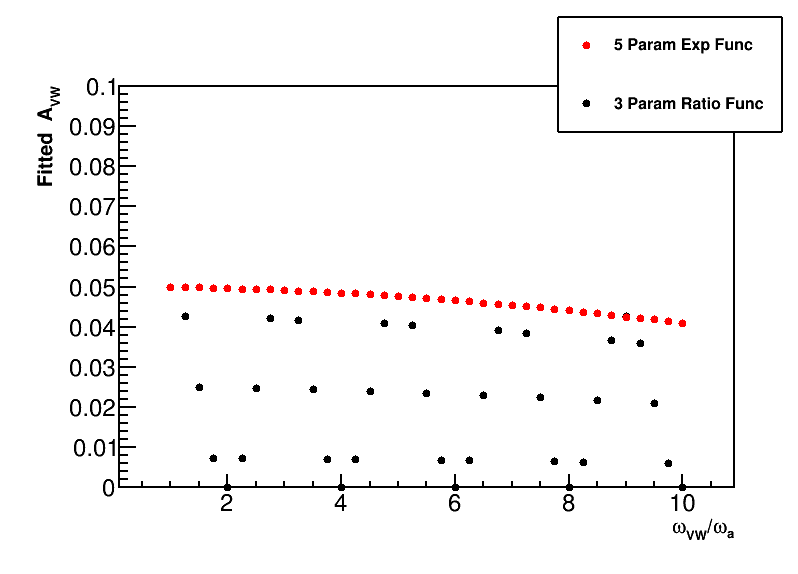
\includegraphics[width=.8\textwidth]{Fitted_Avw_Vs_Wvw_1x-10x}
%     \caption[]{Fitted VW amplitude in a Toy MC as a function of the VW frequency divided by the \gmtwo frequency. In red are the fitted amplitudes with a simple five parameter function, and in black are the fitted amplitudes with a three parameter ratio function. The input VW amplitude was 0.05, and the VW effect was constant throughout the Toy MC ``fill.'' There is a slight fall off of the red points due to the effects of the higher frequencies interacting with the bin width causing a reduction in the fitted amplitude; if an integral fit is used then this fall off is eliminated. What can be seen is that for even frequencies the VW effect dies away in the ratio fit, while for odd frequencies it does not.}
%     \label{fig:VW1x-10x}
% \end{figure}
% %  \texttt{/gm2/app/users/nkinnaird/RatioAnalysis/gm2Dev\_v9\_21\_03/srcs/gm2analyses/macros/RatioMacro/ToyMC/VW\_MC/OnlyVW/grid/ratioToyHists-OnlyVW-1x-10x-37iters.root}


% \begin{figure}[]
%     \centering
%     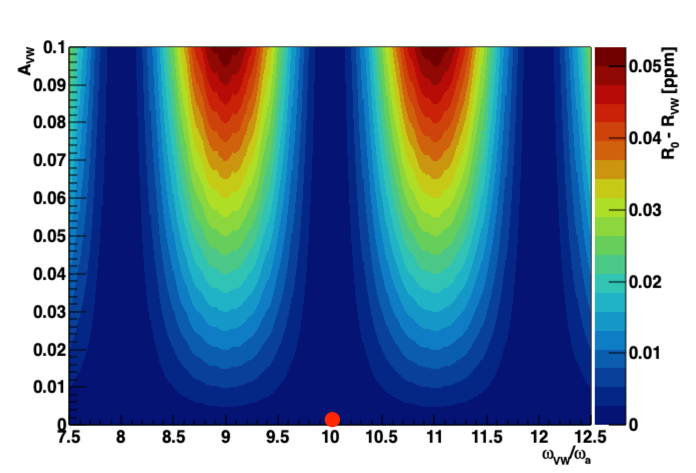
\includegraphics[width=.8\textwidth]{VWRatioDiff}
%     \caption[]{Plotted is the difference in the maximum value of the ratio with and without a VW function included, as a function of both the amplitude of the VW effect and the VW frequency in units of the \gmtwo frequency, in a toy Monte-Carlo simulation. Note that this is not $\boldsymbol{R}$ the frequency fit parameter, but the actual value of the ratio fit function. The difference reaches a minimum for even multiples of the \gmtwo frequency, where the VW effect divides out almost entirely. The $n = 0.108$ datasets, including the 60h and Endgame datasets, live at the bottom center of this plot, marked by a red circle, where the VW frequency is nearly equal to 10 times the \gmtwo frequency, and the difference in the ratio is approximately \SI{5e-6}{} at 30 $\mu s$. Plot courtesy of James Mott.}
%     \label{fig:VWRatioDiff}
% \end{figure}


\begin{figure}[]
\centering
    \begin{subfigure}[t]{0.7\textwidth}
        \centering
        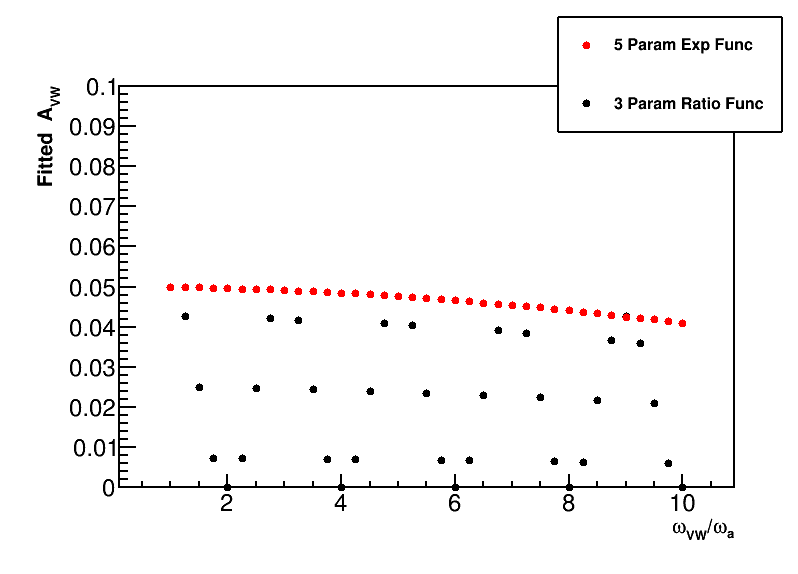
\includegraphics[width=\textwidth]{Fitted_Avw_Vs_Wvw_1x-10x} % \texttt{/gm2/app/users/nkinnaird/RatioAnalysis/gm2Dev\_v9\_21\_03/srcs/gm2analyses/macros/RatioMacro/ToyMC/VW\_MC/OnlyVW/grid/ratioToyHists-OnlyVW-1x-10x-37iters.root}
        \caption{Fitted VW amplitude with a five parameter function in red and a three parameter ratio function in black. The input amplitude was 0.05. The slight fall off of the red points is due to the high frequencies interacting with the bin widths; performing an integral fit removes this trend.}
    \end{subfigure}%

    \begin{subfigure}[t]{0.7\textwidth}
        \centering
        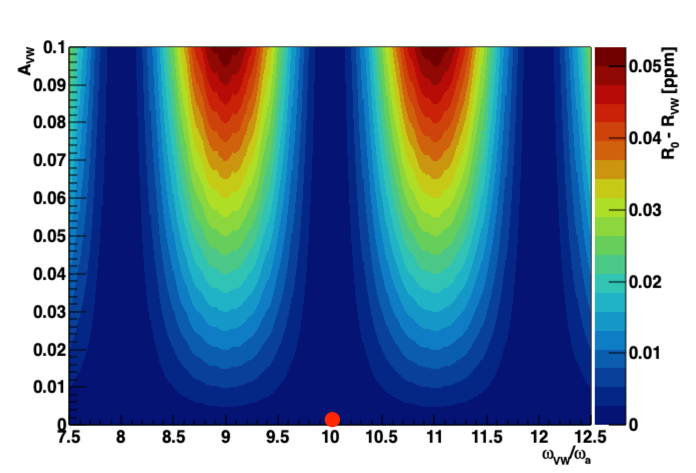
\includegraphics[width=\textwidth]{VWRatioDiff}
        \caption{The difference in the maximum value of the ratio (not the fit parameter \textbf{R}), as a function of VW frequency and amplitude.The difference in the ratio is approximately \SI{5e-6}{} at \mus{30}.}
    \end{subfigure}
\caption[]{Two separate Toy MC simulations showing the division of a VW effect as a function of it's frequency in units of \wa. For even multiple frequencies the effect dies away while for odd multiples it is preserved.}
\label{fig:ToyMCVW}
\end{figure}



\begin{figure}[]
\centering
    \begin{subfigure}[t]{0.7\textwidth}
        \centering
        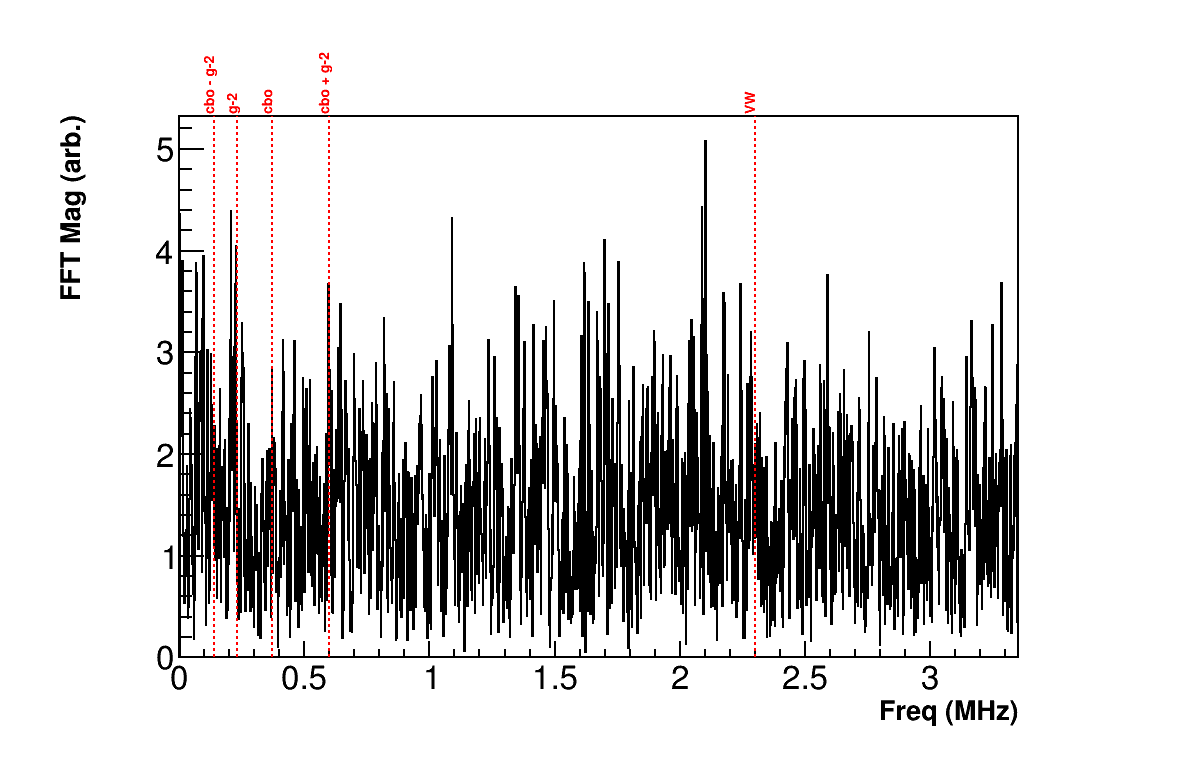
\includegraphics[width=\textwidth]{FFT_3param_allTimes} % From file \texttt{/gm2/data/users/nkinnaird/Ratio/60h-FinalProduction/RandSeeds/FitIterations/output-60h-FinalProduction-RandSeeds-1sttest.root} \texttt{FitPass0}.
        \caption{All times, \SIrange{30.2}{650}{\micro s}.}
    \end{subfigure}%

    \begin{subfigure}[t]{0.7\textwidth}
        \centering
        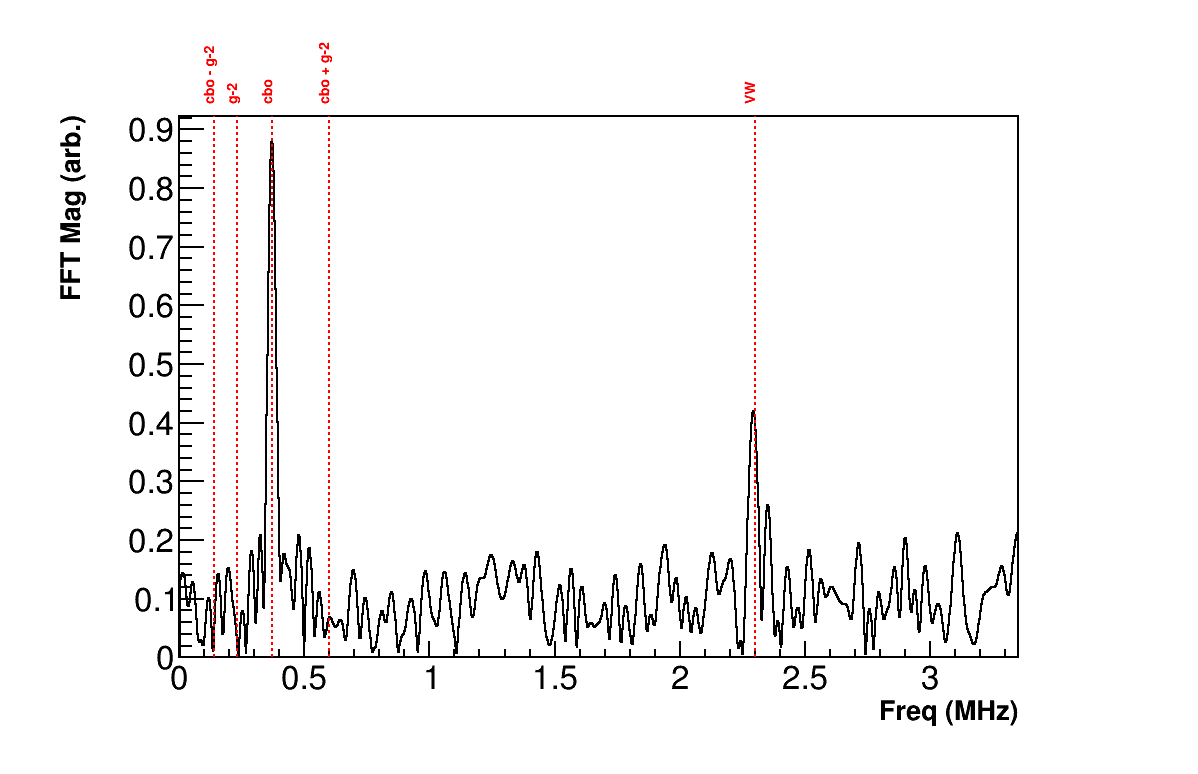
\includegraphics[width=\textwidth]{FFT_3param_earlyTimes} % From file \texttt{/gm2/data/users/nkinnaird/Ratio/60h-FinalProduction/RandSeeds/FitIterations/output-60h-FinalProduction-RandSeeds-1sttest.root} \texttt{FitPass0}.
        \caption{Early times, \SIrange{30.2}{60.2}{\micro s}.}
    \end{subfigure}
\caption[]{FFT of fit residuals using a 3 parameter ratio function to fit the 60h dataset. Peaks can be seen when looking at fit residuals over early times as opposed to all times. The size of the VW peak greatly depends on the choice of random seed. The CBO peak can also be seen.}
\label{fig:FFT_3param}
\end{figure}


\begin{figure}[]
    \centering
    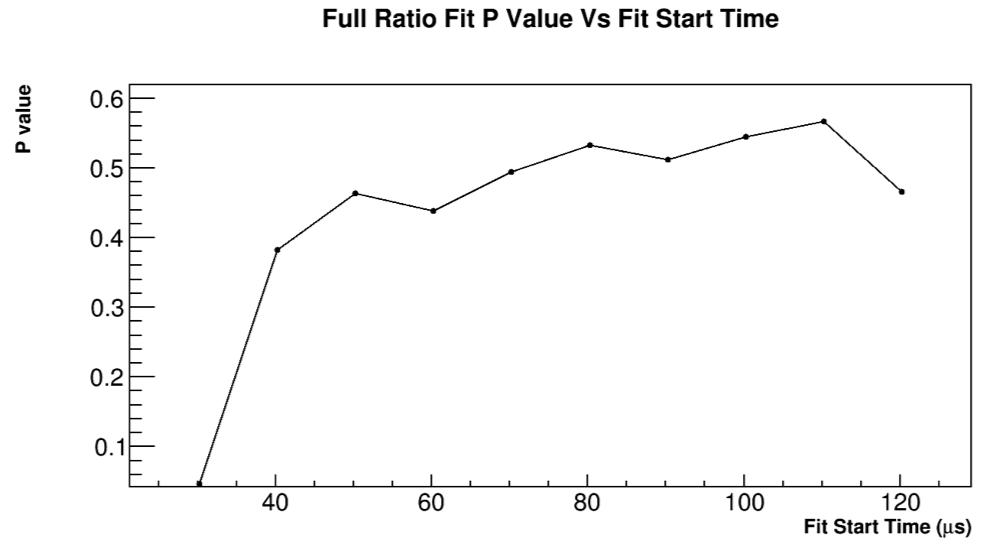
\includegraphics[width=.7\textwidth]{Pvalue_Endgame}
    \caption[]{P value vs fit start time for the Endgame dataset. A sharp rise can be seen at early times. A similar trend, though less severe, can be seen for the 60h dataset.}
    \label{fig:Pvalue_Endgame}
\end{figure}



\section{On a resonance in the 60h and Endgame datasets}

When the VW is included in the ratio fit for the 60h and Endgame results, the resulting fitted VW amplitude is signifcantly larger than that in the T Method, $A_{VW-R} \sim 0.2 \pm 0.04$ vs $A_{VW-T} \sim 0.003 \pm 0.003$ vs. See \figref{fig:60hfitsVW}. This amplitude rises to values 10 to 100 times larger than that in the T Method (depending on random seed) to levels which would naively seem to be directly observable by eye in the data. Interestingly enough, it is only when VW amplitude in the ratio fit is allowed to float that the VW FFT peak disappears and the fit start scans are repaired. The fit does truly seem to prefer such a large value, however this was an anomaly which needed to be understood.


\begin{figure}[]
\centering
    \begin{subfigure}[]{0.8\textwidth}
        \centering
        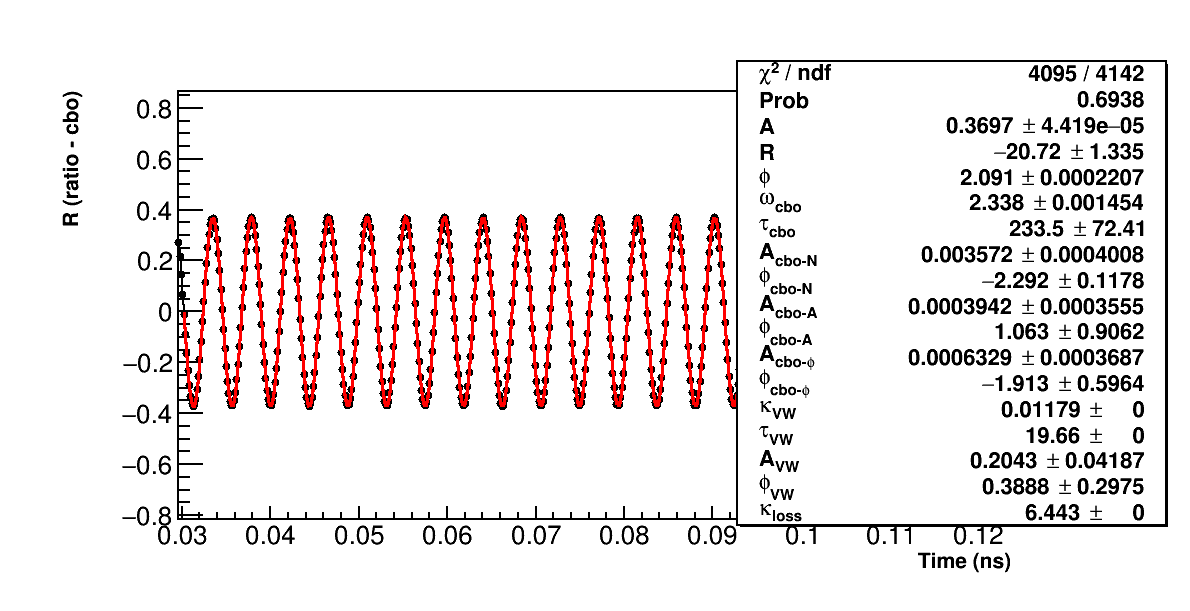
\includegraphics[width=\textwidth]{ratioFit_highVWamp}
        \caption{Ratio Method fit results with the VW included.}
    \label{fig:ratioFit_highVWamp}
    \end{subfigure}%
    \vspace{1cm}
    \begin{subfigure}[]{0.8\textwidth}
        \centering
        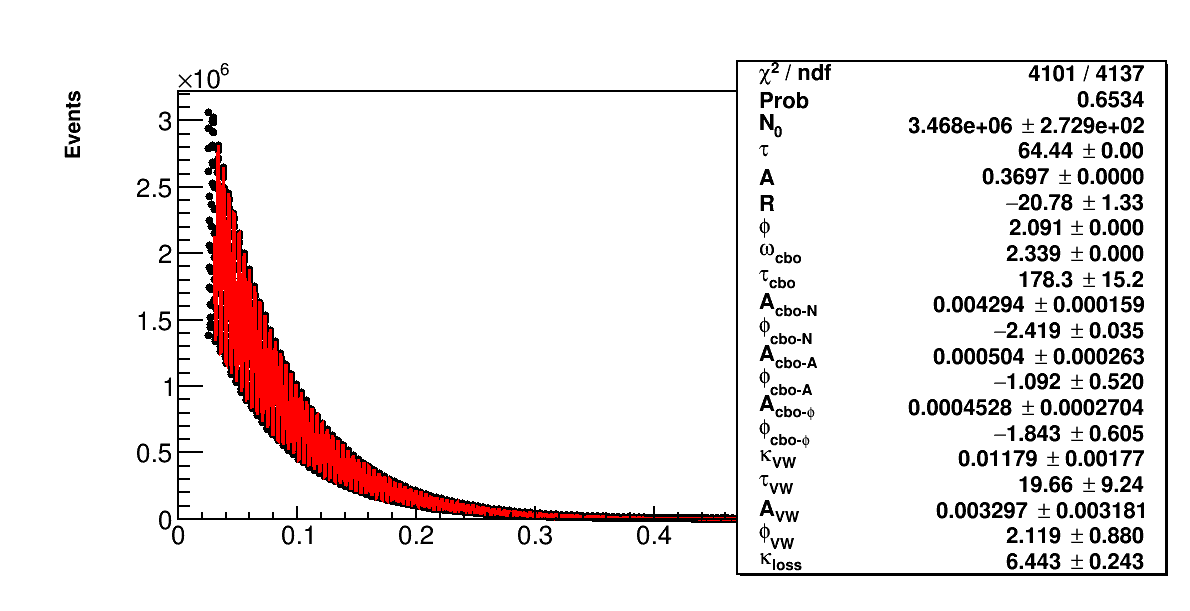
\includegraphics[width=\textwidth]{TmethodFit_lowVWamp}
        \caption{T Method fit results.}
    \label{fig:TmethodFit_lowVWamp}
    \end{subfigure}
\caption[]{Fits to the 60h dataset with the VW included in the ratio fit. The VW frequency and lifetime in the ratio fit are fixed to those determined from the T Method fit, as it can struggle with those parameters, while the amplitude and phase are allowed to float. Comparing the VW fitted amplitudes, the amplitude in the ratio fit is significantly larger.}
\label{fig:60hfitsVW}
\end{figure}
% \texttt{/gm2/data/users/nkinnaird/Ratio/60h-FinalProduction/RandSeeds/FitIterations/output-60h-FinalProduction-RandSeeds-1sttest.root} \texttt{FitPass0}



One possibility considered was whether the ratio fit artificially raises the VW amplitude, and whether a different fit function should be used. Fits were done with the three parameter ratio function,
    \begin{align} \label{eq:threeparamratio}
        R(t) \approx A \cos(\omega_{a}t),
    \end{align}
as well as the full fit function,
    \begin{gather}
        R(t) = \frac{2f(t) - f_{+}(t) - f_{-}(t)}{2f(t) + f_{+}(t) + f_{-}(t)}, \\
        f_{\pm}(t) = f(t \pm T_{a}/2), \\
        f(t) = V(t) \cdot (1 + A \cdot \cos(\omega_{a}t + \phi)),
    \label{eq:fullratiofunction}
    \end{gather}
where $V(t)$ is the vertical waist effect. In the latter, $f(t)$ represents the same function used in a 5 parameter or T Method fit function, barring the $N_{0}$ and $\tau_{\mu}$ terms which divide out. Fitting the Toy MC simulated data with these functions yielded the results shown in \figref{fig:FittedAVW_myToyMC}. For the three parameter function fits, it can be seen that the VW effect dies away as the frequency approaches 10 times \wa. For the full ratio function results however, it can be seen that the fitted VW amplitudes start to vary with large errors, typically consistent with zero. This effect makes sense, as while the VW effect has been removed from the ratio data, but the fit parameter gets divided out in the fit function, and so can be any value while still giving the same goodness of fit. The instability of this fit parameter (and it's demotivation), was originally thought to be the source of the large amplitudes in the fit to the data. However, regardless of the way the dataset was sliced, and regardless of whether the 60h or Endgame was fit, the fits always preferred a large amplitude with a relatively small error.



\begin{figure}[]
\centering
    \begin{subfigure}[]{0.46\textwidth}
        \centering
        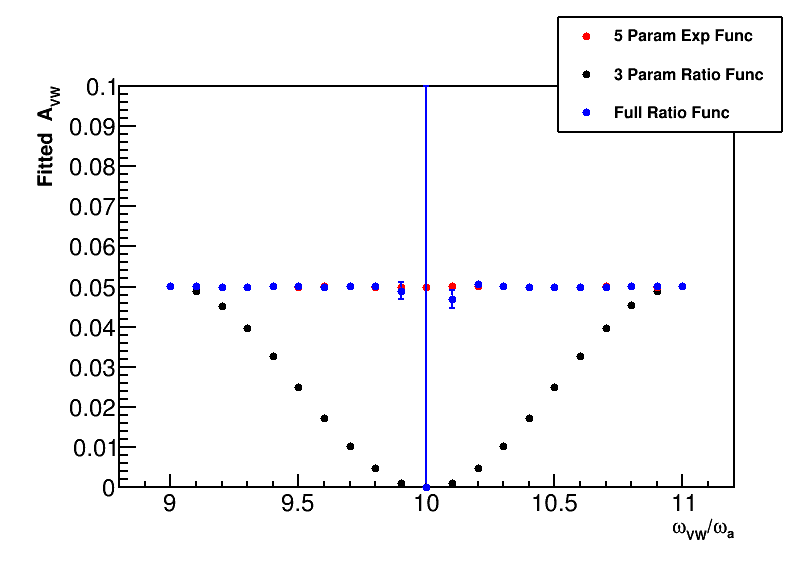
\includegraphics[width=\textwidth]{Fitted_Avw_Vs_Wvw-9x-10x}
        \caption{$9\times$ to $11\times$ \wa.}
    \end{subfigure}% %you need this % here to add spacing between subfigures
    \hspace{1cm}
    \begin{subfigure}[]{0.46\textwidth}
        \centering
        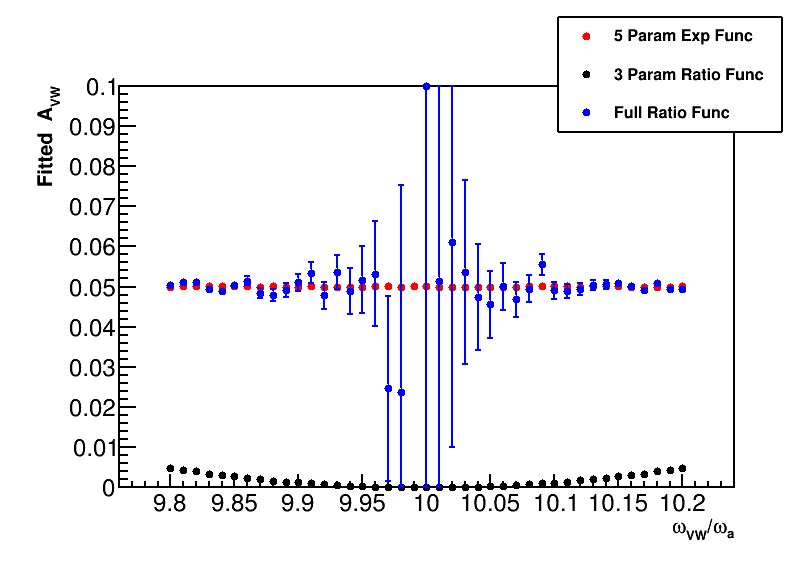
\includegraphics[width=\textwidth]{Fitted_Avw_Vs_Wvw-10x}
        \caption{$9.8\times$ to $10.2\times$ \wa.}
    \end{subfigure}
\caption[]{Fitted VW amplitude as a function of frequency and with different types of fit functions. }
\label{fig:FittedAVW_myToyMC}
\end{figure}
% \texttt{/gm2/app/users/nkinnaird/RatioAnalysis/gm2Dev\_v9\_21\_03/srcs/gm2analyses/macros/RatioMacro/ToyMC/VW\_MC/OnlyVW/grid/ratioStyleFunc}



Therefore a more data-like Toy MC simulation was built which included the FR effect, with the ability to turn off various parts of the simulation. It was found that when the FR was turned off the ratio data was consistent with 0, while when the FR was turned on, the VW effect reappeared with a larger amplitude and a strange beating structure, \figref{fig:JamesMC_VW_FR}. A simpler Mathematica simulation revealed the same behavior with the same beating structure, \figref{fig:MathematicaMC_VW_FR}. So something in the way that the Ratio Method was interacting with the FR was causing these large amplitudes. Performing the Ratio Method analysis, but this time with varying time-shifts, revealed the resonance very clearly in both the data and the Mathematica simulation, \figref{fig:resonance}. As shown the running point for 60h and Endgame datasets sits on this resonance, stemming from the fact that $f_{VW} \approx 10 \cdot f_{a}$. This begs the questions as to what exactly is the source of this resonance, and how exactly does the Ratio Method introduce it in combination with the FR.


\begin{figure}[]
\centering
    \begin{subfigure}[t]{0.7\textwidth}
        \centering
        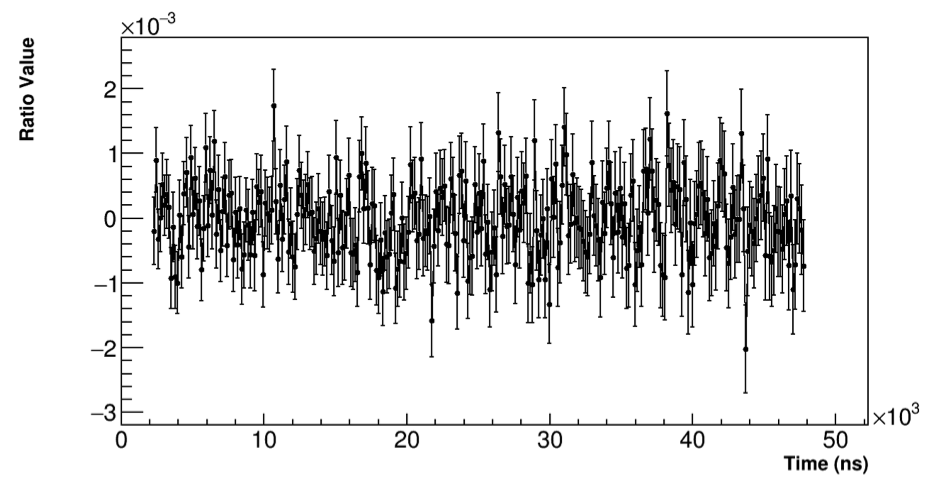
\includegraphics[width=\textwidth]{JamesMC_noFR}
        \caption{Without the FR effect included.}
    \end{subfigure}%

    \begin{subfigure}[t]{0.7\textwidth}
        \centering
        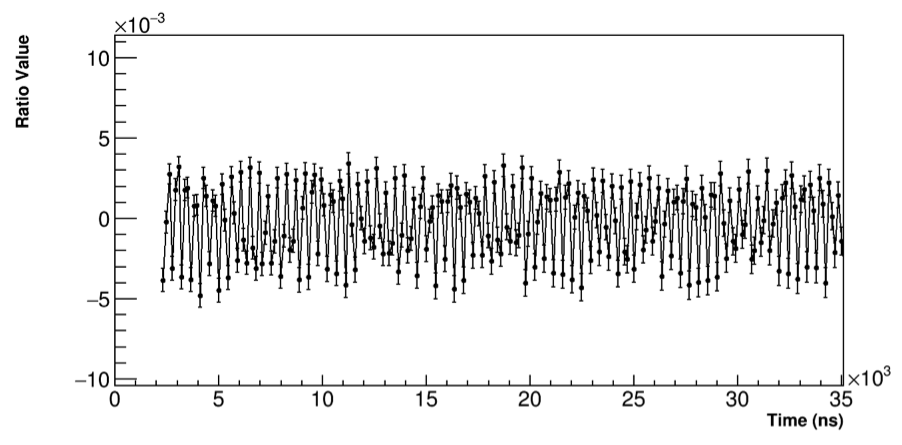
\includegraphics[width=\textwidth]{JamesMC_withFR}
        \caption{With the FR effect included.}
    \end{subfigure}
\caption[]{Ratio data with and without the FR effect from a Toy MC simulation, with a VW effect with a frequency $f_{VW} = 10 \cdot \omega_{a}$. The \gmtwo wiggle has been removed, and the lifetime of the VW was set to a large number. The top plot shows ratio data which is consistent with 0 after all effects have been removed and the VW has divided out. The bottom plot shows ratio data inconsistent with 0, with oscillations at the VW frequency, and an interesting beating structure.}
\label{fig:JamesMC_VW_FR}
\end{figure}


\begin{figure}[]
\centering
    \begin{subfigure}[t]{0.7\textwidth}
        \centering
        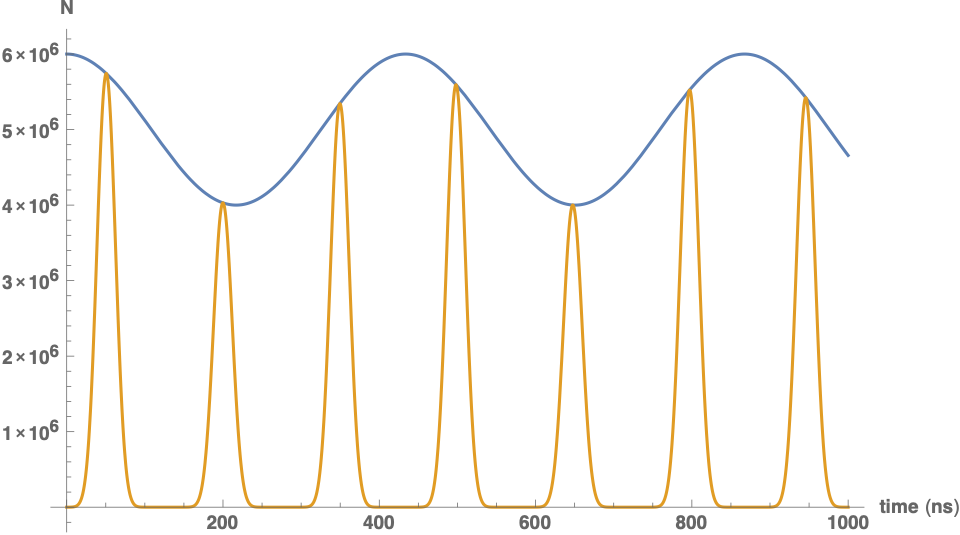
\includegraphics[width=\textwidth]{MathematicaMC_functionExample}
        \caption{The input functions used, blue for the VW and orange for a FR effect.}
    \end{subfigure}%
    \vspace{1cm}
    \begin{subfigure}[t]{0.7\textwidth}
        \centering
        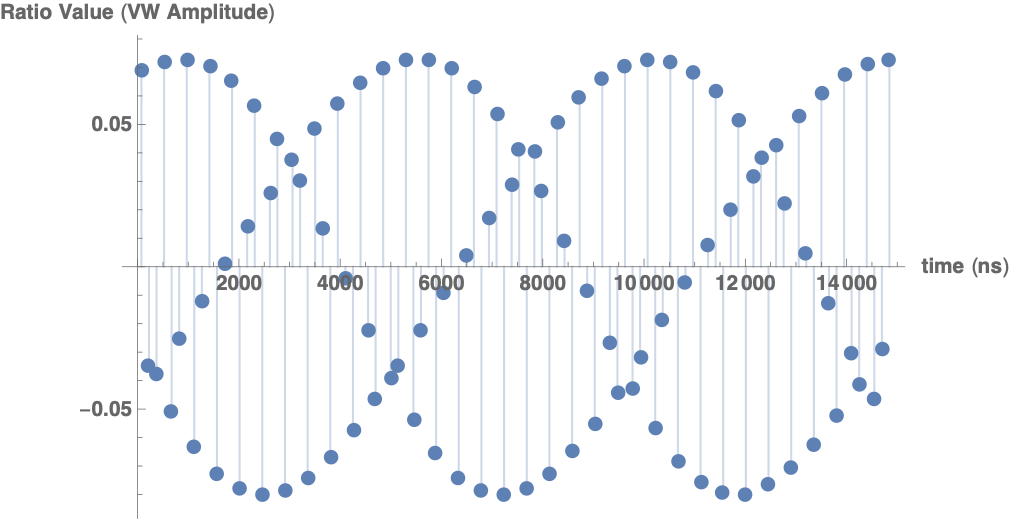
\includegraphics[width=\textwidth]{MathematicaMC_withFR}
        \caption{The ratio value with the FR effect include. Oscillations with large amplitudes at the VW frequency can be seen with the same strange beating structure.}
    \end{subfigure}
\caption[]{Results from a simple Mathematica simulation with a VW and FR effect included.}
\label{fig:MathematicaMC_VW_FR}
\end{figure}


\begin{figure}[]
\centering
    \begin{subfigure}[t]{0.8\textwidth}
        \centering
        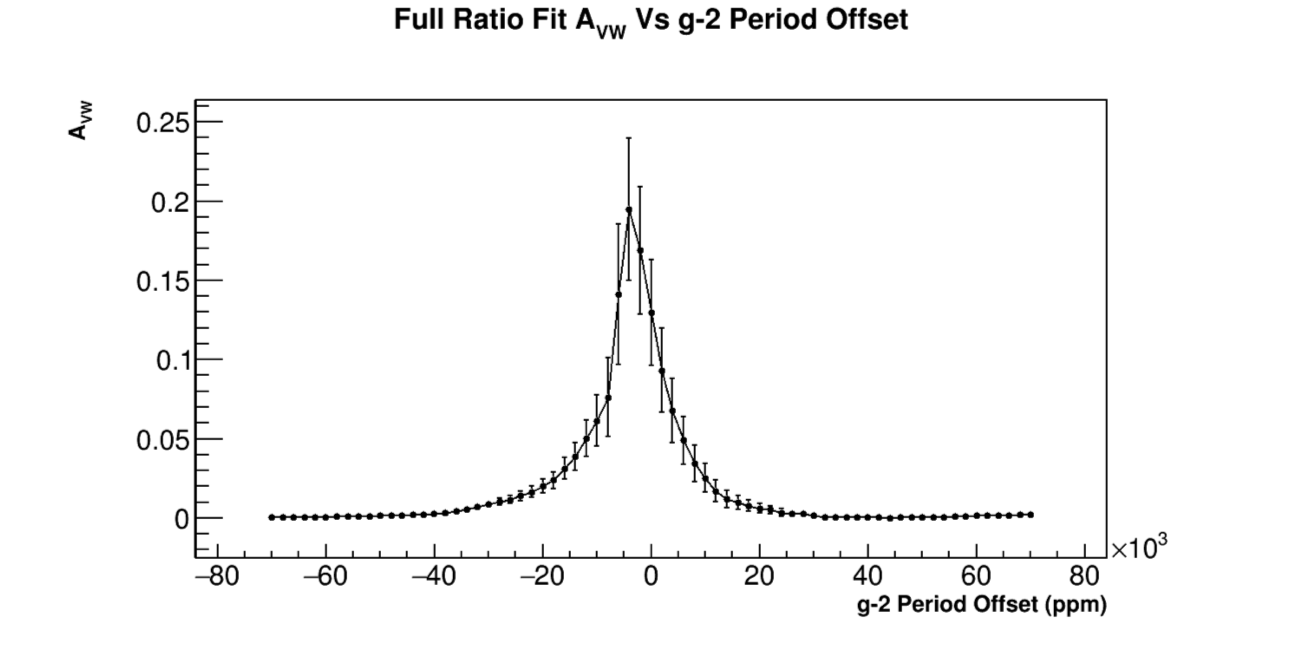
\includegraphics[width=\textwidth]{AvwResonance_60h}
        \caption{Fitted VW amplitude as a function of the choice of \gmtwo period offset in units of thousands of ppm for the 60h dataset.}
    \end{subfigure}%
    \vspace{1cm}
    \begin{subfigure}[t]{0.6\textwidth}
        \centering
        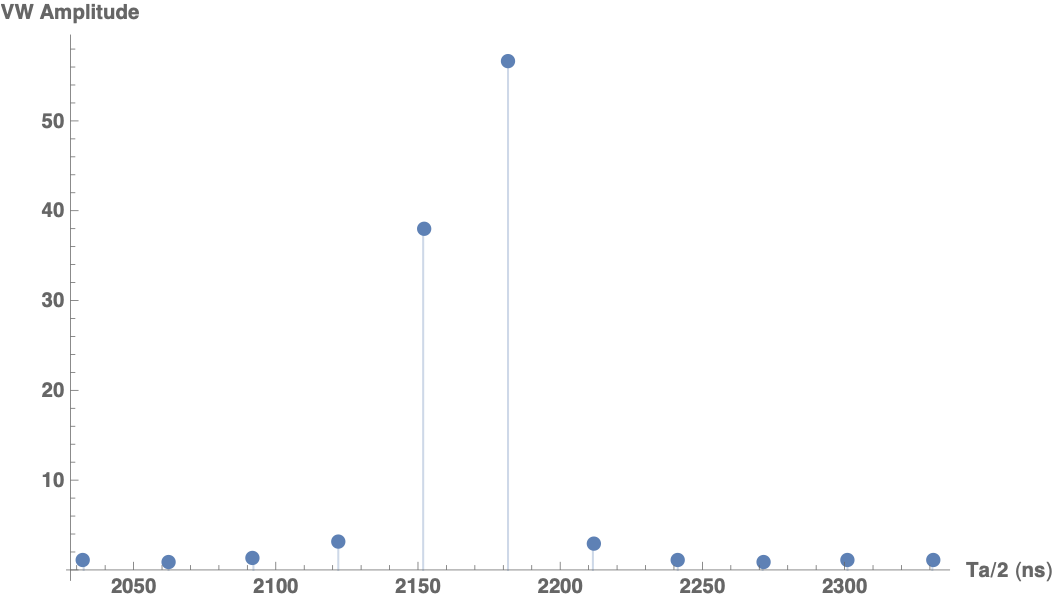
\includegraphics[width=\textwidth]{AvwResonance_Mathematica}
        \caption{Fitted VW amplitude as a function of the choice of \gmtwo period in the Mathematica simulation.}
    \end{subfigure}
\caption[]{The amplitude of the fitted VW, in both the data (top) and Mathematic simulation (bottom), as a function of the time-shift or \gmtwo period over 2, $T_{a}/2$. In both the resonace can be clearly seen where the VW amplitude blows up from it's real value.}
\label{fig:resonance}
\end{figure}


With yet another Toy MC, the resonances in the VW amplitude can be seen as a function of the time shift over the VW period, \figref{fig:JamesAnalytic_Avw_Resonances}. As shown the resonances appear at integer steps in the time shift over the VW period. Let's determine why these resonances appear by looking at the ratio fit function more carefully as a function of the time shift. The explicit ratio function is given as \cite{60hReport}
    \begin{align}
        R(t) = \frac{2 A \cos(\omega_{a}t) (1 - \cos{(\omega_{a}\Delta)})} {4 + 2A \cos(\omega_{a}t) (1 + \cos{(\omega_{a}\Delta)} )},
    \end{align}
where $\Delta$ is the time shift, typically 
    \begin{align}
        \Delta \approx T_{a}/2.
    \end{align}
In the Toy MC the \wa oscillation was removed and replaced with a VW oscillation, so the ratio function instead goes as 
    \begin{align}
        R(t) = \frac{2 A \cos(\omega_{VW}t) (1 - \cos{(\omega_{VW}\Delta)})} {4 + 2A \cos(\omega_{VW}t) (1 + \cos{(\omega_{VW}\Delta)} )},
    \end{align}
where \wa has simply been replaced by $\omega_{VW}$. Looking at the numerator of this function, it can be seen that the numerator goes to zero when 
    \begin{align}
        \Delta = 2n\pi/\omega_{VW} = n \cdot T_{VW},
    \end{align}
at integer steps in the time shift over the VW period. This can be seen in \figref{fig:ratiofunc_analytic}. When looking at the real simulated data however, including the effects of the FR, as shown in \figref{fig:ratiofunc_data}, it can be seen that the real ratio data does not in fact go to zero. This is in fact the root cause for the VW amplitude resonances. Because the ratio function is going to zero at points where the real data is non-zero, the VW amplitude in the fit function explodes to compensate for the wrong fit function form. Note that this large amplitude does not mean that there is a correspondingly large wiggle in the data, as this frequency is still close to an even multiple and will thus divide out, but the higher amplitude does produce greater agreement between the data and the fit function. While technically this means that the VW envelope used in the fit function is wrong for fitting the data and the Toy MC, the VW effect is small enough and the frequency is close enough to an even multiple that fits still retain good goodness of fit. To solve this issue, even though the goodness of fit is good since the VW effect is small, either the real envelope should be incorporated in the fit, or the VW should be eliminated. The former is not simple, as the envelope shown in \figref{fig:JamesMC_VW_FR} is complicated. The latter approach was chosen, as will be described in Section~\ref{sec:randomization}.



\begin{figure}[]
    \centering
    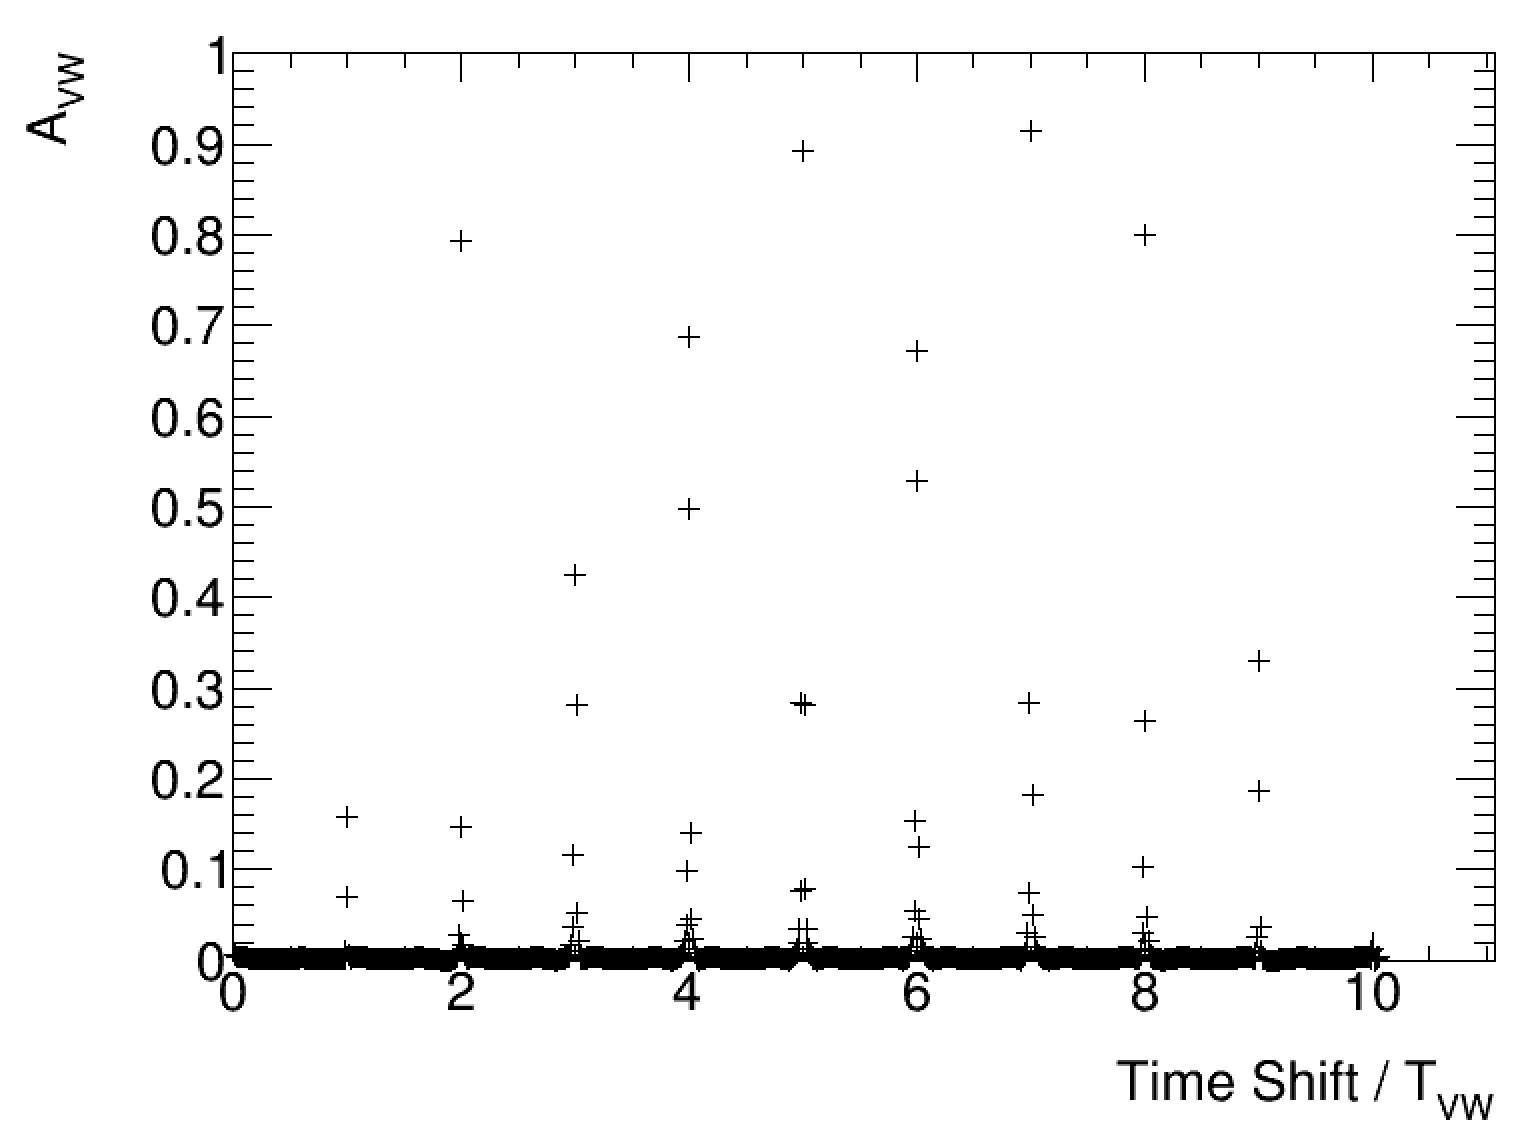
\includegraphics[width=.7\textwidth]{JamesAnalytic_Avw_Resonances}
    \caption[]{VW amplitude resonances as a function of the time shift in the Ratio Method divided by the VW period, $T_{VW}$.}
    \label{fig:JamesAnalytic_Avw_Resonances}
\end{figure}



\begin{figure}[]
\centering
    \begin{subfigure}[t]{0.7\textwidth}
        \centering
        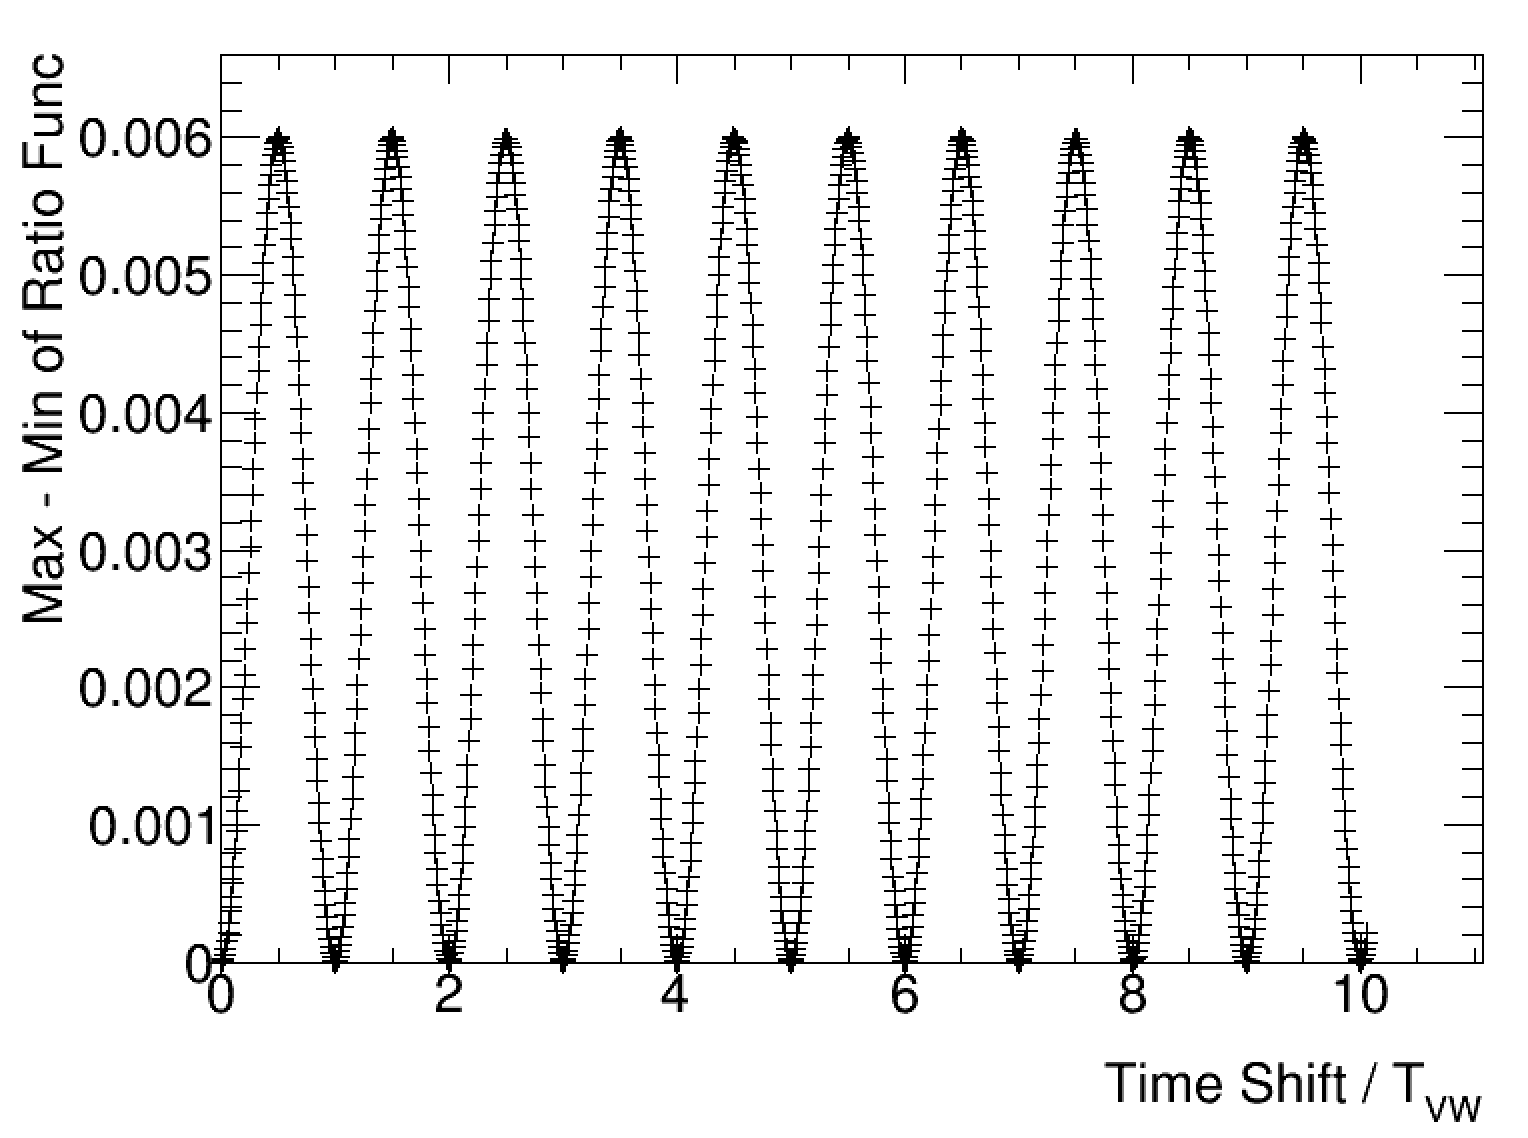
\includegraphics[width=\textwidth]{JamesAnalytic_RatioAmp_noFR}
        \caption{At integer steps in the time shift over the VW period the amplitude of the ratio fit function goes to zero.}
    \label{fig:ratiofunc_analytic}
    \end{subfigure}%
    \vspace{5mm}
    \begin{subfigure}[t]{0.7\textwidth}
        \centering
        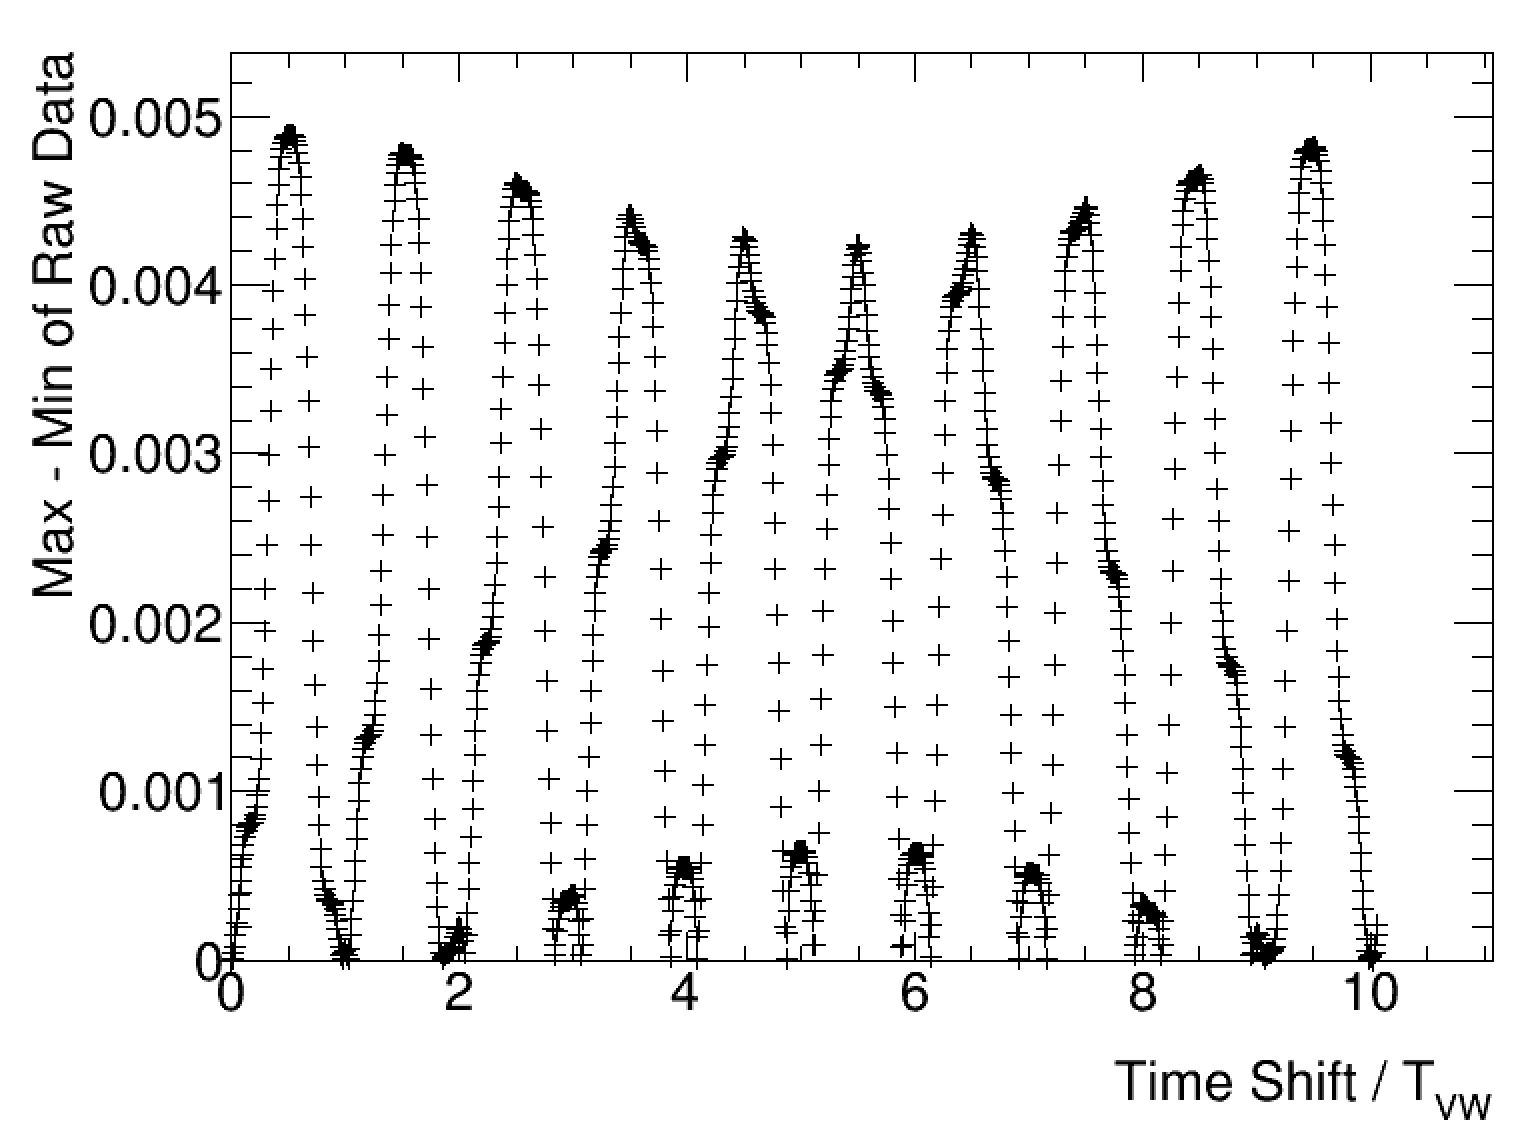
\includegraphics[width=\textwidth]{JamesAnalytic_RatioAmp_withFR}
        \caption{At integer steps in the time shift over the VW period the amplitude of the ratio data does not go to zero, due to the existence of the FR effect.}
    \label{fig:ratiofunc_data}
    \end{subfigure}
\caption[]{The maximum amplitude of the ratio function (top) and Toy MC ratio data (bottom), as a function of the time shift divided by the VW period.}
\label{fig:ratiofunc_compare}
\end{figure}





\clearpage






\section{9d Dataset - a different problem}


While in the 60h and Endgame datasets the VW frequency is nearly 10 times \wa, in the 9d the frequency is closer to an odd multiple, or $\omega_{VW} \approx 8.87 \cdot \omega_{a}$ at $t = \infty$. With what I've shown so far, I expect the VW signal to be easily fittable with an amplitude equal to that from the T method results. Looking at per calo fit results in \figref{fig:9d-PerCalo-VW}, the VW phases and amplitudes are consistent between the T method and ratio method results. As shown there are no observable differences. When I look at the fits to the sum of the calorimeter data however, I see a systematically smaller VW amplitude in the ratio fit results as compared to the T method results. This is true for all random seeds as shown in \figref{fig:vw-fixed-w-tau-9d-randseeds}. While I expect a reduction in the VW amplitude from per calo fits to the calorimeter sum fit, as the phases go from 0-2$\pi$ around the ring, I still expect the amplitudes to be consistent between the T method and ratio method. If I take calorimeters adjacent to each other around the ring versus calorimeters separated from each other, then I see the behaviour. So what seems to be happening is that there is a cancellation when adding the calorimeters together in the ratio method that doesn't occur in the T method. That is something I don't understand, and can't come up with a reason why that should happen. I'm not sure if this is at all related to the previously discussed problem or not, whether it's another symptom or something else strange. 



\begin{figure}[]
\centering
    \begin{subfigure}[]{0.46\textwidth}
        \centering
        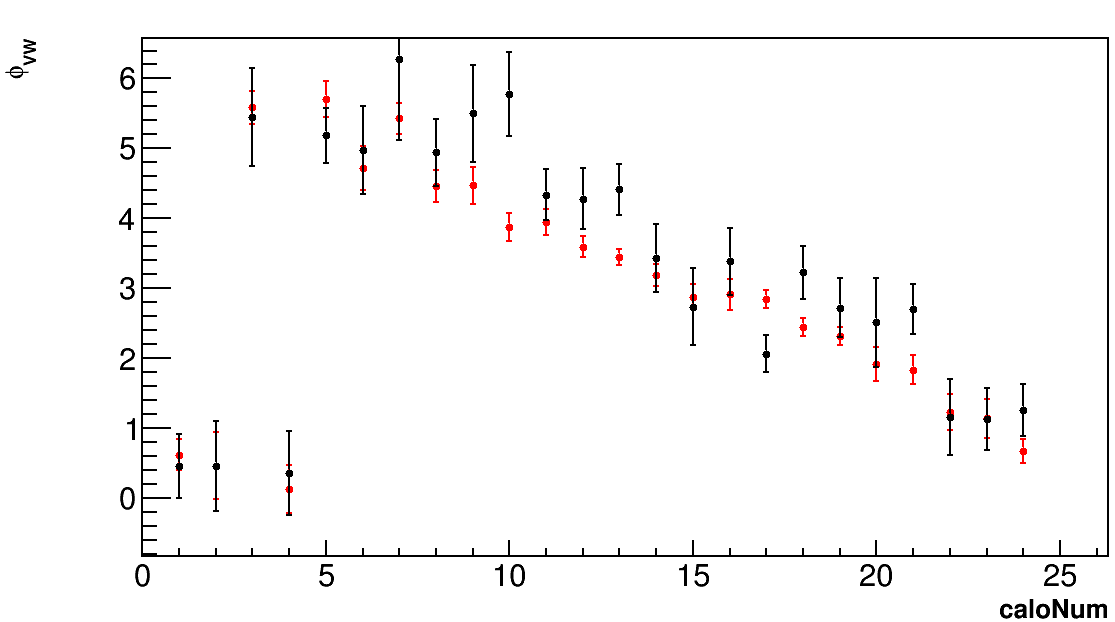
\includegraphics[width=\textwidth]{9d-CaloFits-VW-Phases}
        \caption{VW phases per calo in the 9d dataset.}
    \end{subfigure}% %you need this % here to add spacing between subfigures
    \begin{subfigure}[]{0.46\textwidth}
        \centering
        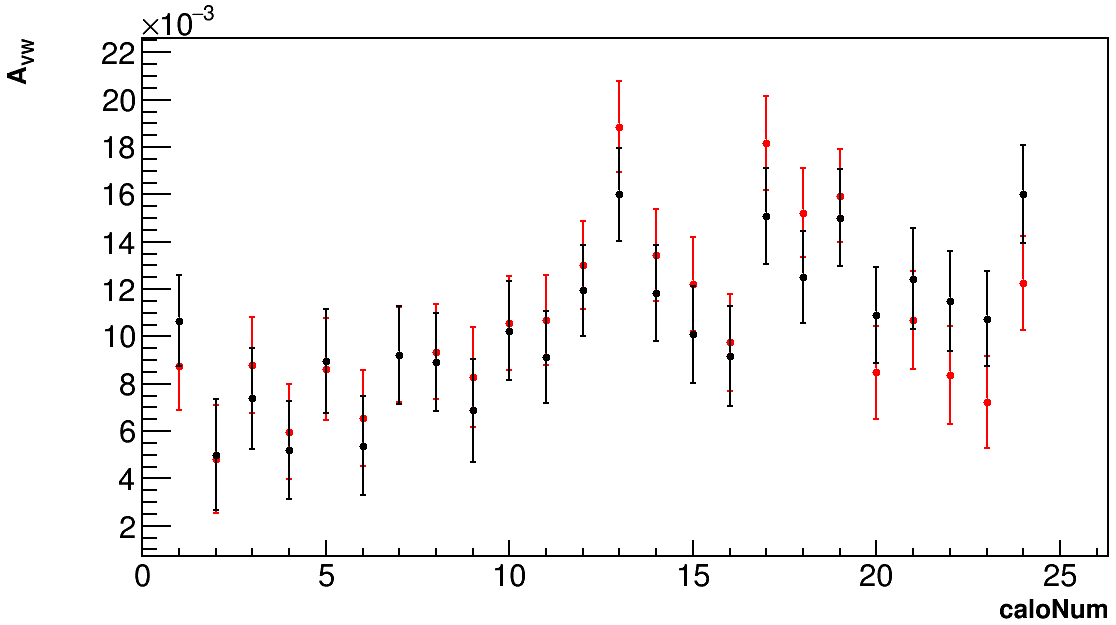
\includegraphics[width=\textwidth]{9d-CaloFits-VW-Amps}
        \caption{VW amplitudes per calo in the 9d dataset.}
    \end{subfigure}
\caption[]{Red points are T method results and black points are ratio method results. In the ratio fits, the VW frequencies and lifetimes are fixed to those from the T method results.}
\label{fig:9d-PerCalo-VW}
\end{figure}
% \texttt{/gm2/data/users/nkinnaird/Ratio/9d-FinalProduction/SingleIteration/temptests/CaloFits-VW-w-tau-fixed}

\begin{figure}[]
    \centering
    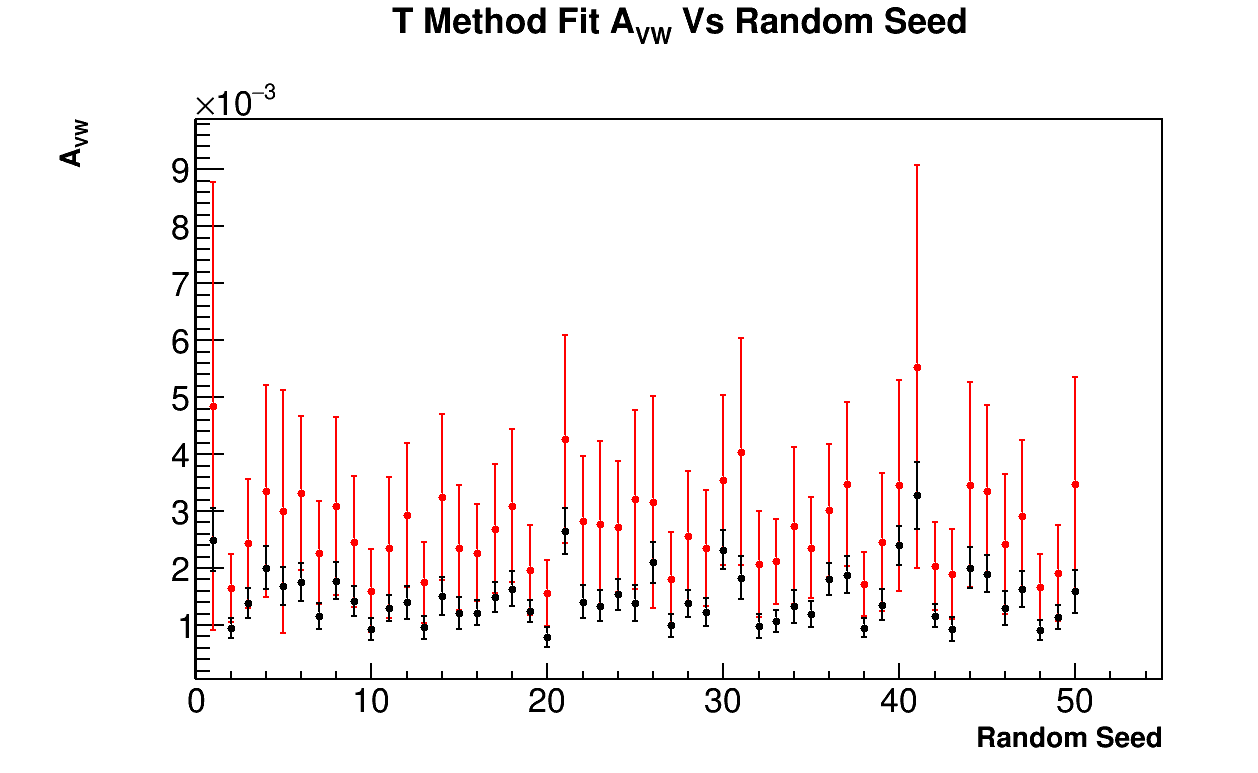
\includegraphics[width=0.7\textwidth]{vw-fixed-w-tau-9d-randseeds}
    \caption[]{VW amplitudes as a function of random seed for T method fits compared to ratio method fits. T method fits are in red and ratio fits are in black. The error bars are smaller on the ratio fits because the VW frequencies and lifetimes are fixed to those from the T method fits. There is a consistently smaller VW amplitude in the ratio fits as compared to the T method fits.}
    \label{fig:vw-fixed-w-tau-9d-randseeds}
\end{figure}
% \texttt{/gm2/data/users/nkinnaird/Ratio/9d-FinalProduction/RandomSeeds/tests\_with\_VW/fixed-vw-w-tau}





\section{Randomizing out the effect...}
\label{sec:randomization}

2fy randomization results are shonw in \cite{wa_presentation}


effects on R...
statisitical error increases by.. 


\begin{table}[]
\centering
\small
\setlength\tabcolsep{10pt}
\renewcommand{\arraystretch}{1.2}
\begin{tabular*}{1\linewidth}{@{\extracolsep{\fill}}lcccccB}
  \hline
    \multicolumn{7}{c}{\textbf{R Comparison with and without Randomization}} \\
  \hline\hline
    & & \multicolumn{2}{c}{With VW} & \multicolumn{2}{c}{Without VW} & \\
    & & \multicolumn{2}{c}{No Randomization} & \multicolumn{2}{c}{With Randomization} & \\
  \hline\hline
    Dataset & Fit Method & Mean & RMS & Mean & RMS & \thead{$\Delta R$} \\
  \hline
    \multirow{2}{*}{60H} & T & $-20.345$ & $0.143$ & $-20.294$ & $0.298$ & 0.051 \\
                         & R & $-20.527$ & $0.216$ & $-20.480$ & $0.357$ & 0.047 \\
  \hline
    \multirow{2}{*}{9d} & T & $-17.278$ & $0.065$ & $-17.280$ & $0.126$ & -0.002 \\
                        & R & $-17.355$ & $0.087$ & $-17.374$ & $0.133$ & -0.019 \\
  \hline
    \multirow{2}{*}{Endgame} & T & $-17.743$ & $0.096$ & $-17.684$ & $0.186$ & 0.059 \\
                             & R & $-17.747$ & $0.125$ & $-17.688$ & $0.192$ & 0.059 \\                                              
  \hline
\end{tabular*}
\caption[]{Means and RMS' of R values for 50 different random seeds for three of the Run~1 datasets, without the $f_{VW}$ randomization and including the VW in the fit, versus with the $f_{VW}$ randomization and the VW terms excluded from the fit.}
\label{tab:fVW_Randomization}
\end{table}







\printbibliography



% \begin{figure}[]
%     \centering
%     \includegraphics[width=\textwidth]{}
%     \caption[]{}
%     \label{fig:}
% \end{figure}


% \begin{figure}[]
% \centering
%     \begin{subfigure}[t]{0.7\textwidth}
%         \centering
%         \includegraphics[width=\textwidth]{}
%         \caption{}
%     \end{subfigure}%

%     \begin{subfigure}[t]{0.7\textwidth}
%         \centering
%         \includegraphics[width=\textwidth]{}
%         \caption{}
%     \end{subfigure}
% \caption[]{}
% \label{}
% \end{figure}


\end{document}

